\documentclass[a4paper,11pt,twocolumn]{article}
\input{structure.tex}

\begin{document}
{\huge \textbf{Geomeetrilised konstruktsioonid optikas}\hfill \normalsize{nr 8}} \\
{Kaarel Kivisalu \hfill 26. märts 2019}

Läätsede jaoks kehtivad järgnevad kasulikud omadused:
\begin{itemize}
\item läätse keskpunkti läbiv kiir ei murdu;
\item optilise teljega paralleelne kiir (või tema pikendus) läbib fookust;
\item parallsed kiired koonduvad fokaaltasandil;
\item tasandi kujutis läbi läätse on tasand, sirge kujutis on sirge ja punkti kujutis on punkt;
\item sirge ja tema kujutise pikendused lõikuvad läätse tasandil.
\end{itemize}

% Õhukese läätse valem (olge märkidega hoolikad):
% \begin{equation*}
%   \frac{1}{a} + \frac{1}{k} = \frac{1}{f}
% \end{equation*}

\begin{question}[Lõppv 2018, G1][gop3][7cm]
  Kersti paneb kokku optilise skeemi, nii et koondav lääts on
  objektist ja ekraanist, kuhu terav kujutis tekib, võrdsel
  kaugusel. Ta jätab objekti ja ekraani asukoha samaks, kuid lõikab
  läätse optilise peatelje juurest pooleks ning nihutab kaks tekkinud
  poolikut läätse optilisest peateljest eemale. Joonistage lisalehel
  uue skeemi jaoks kiirte käik. Objekt on tähistatud A-ga.
\end{question}

\begin{question}[Lahtine 2015, V5][gop1][7cm]
  Joonisel on kujutatud objekt $AB$ ning sellest kumerläätses tekkinud
  tõeline kujutis $AʼBʼ$. Leidke konstrueerimise teel läätse
  keskpunkti ning fookuse asukoht.
\end{question}

\begin{question}[Lahtine 2014, V7][gop2][\columnwidth]
  Kõrvaloleval joonisel on kujutatud kahe algselt paralleelse kiire
  käik läbi kahe ühesuguse kumerläätse, mis ei asetse
  paralleelselt. Läätsede fookused ühtivad ning asuvad punktis
  $F$. Konstrueerige skeemile läätsed koos optiliste peatelgedega.
\end{question}

\begin{question}[Lõppv 2016, G8][gop4][3cm]
  Jukul oli katsetamiseks kolm ruudukujulist tasapeeglit. Ühte
  peeglisse vaadates ja paremat silma kinni pigistades nägi ta endast
  joonisel kujutatud peegelpilti. Järgmisena paigutas Juku kolm
  peeglit sedasi, et need moodustasid kuubi kolm tahku, millel on üks
  ühine tipp. Sealjuures jäid peegelpinnad kuubi sisemisele
  poolele. Joonistage peegelpilt, mida paremat silma kinni pigistav
  Juku endast otse nurgapeegli nurka vaadates nägi ja põhjendage
  tulemust konstrueerimise teel.
\end{question}

\begin{question}[Lõppv 2015, G7][gop5][7cm]
  Juuresoleval joonisel on kujutatud ring ja sellest koondava läätse
  poolt tekitatud kujutis. Leidke läätse keskpunkt, optiline peatelg
  ja fookus.
\end{question}

\begin{question}[PhysCup 2012, P7]
  Juuresoleval joonisel kujutatud nelinurk on ruudu tegelik kujutis
  õhukeses ideaalses läätses. Nelinurk ja optiline peatelg asuvad
  joonise tasandis. Rekonstrueeri läätse asukoht (st keskpunkti
  asukoht ja orientatsioon).
\end{question}
\begin{figure}[h!]
    \centering
    \vspace{-1em}
    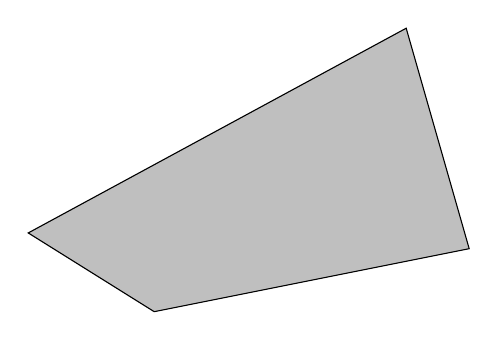
\begin{tikzpicture}[scale=0.4]
        \filldraw[fill=lightgray] (4,0)--(14,2)--(12,9)--(0,2.5)--(4,0);
    \end{tikzpicture}
\end{figure}


\begin{question}[PhysCup 2017, P4][gop7][8cm]
  Juuresoleval joonisel on kujutatud ellips on ringi kujutis õhukeses
  ideaalses läätses. Punkt ellipsi sees kujutab ringi keskpunkti
  kujutist. Ellips ja optiline peatelg asuvad joonise
  tasandis. Rekonstrueeri läätse asukoht (st keskpunkti asukoht ja
  orientatsioon).
\end{question}

%\clearpage
%
%\vspace*{2cm}
%
%\begin{figure}[h]
%    \includegraphics[width=\textwidth]{gop2.pdf}
%    \centering
%    \vspace{-1em}
%\end{figure}
%
%\begin{figure}[h]
%    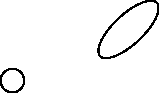
\includegraphics[width=\textwidth]{gop5.pdf}
%    \centering
%    \vspace{-1em}
%\end{figure}

\end{document}
